\documentclass[DIV=calc, paper=a4, fontsize=11pt, twocolumn]{scrartcl}

%-------------------------------------------------
%   THEMES, PACKAGES, CUSTOM COMMANDS
%-------------------------------------------------
\usepackage{blindtext}
\usepackage[english]{babel}                             % English language/hyphenation
\usepackage[protrusion=true,expansion=true]{microtype}  % Better typography
\usepackage{amsmath,amsfonts,amsthm}                    % Math packages
\usepackage[pdftex]{graphicx}                           % Enable pdflatex
\usepackage[svgnames]{xcolor}                           % Enabling colors by their 'svgnames'
\usepackage[hang, small,labelfont=bf,up,textfont=it,up]{caption} % Custom captions under/above floats
\usepackage{epstopdf}       % Converts .eps to .pdf
\usepackage{subfig}         % Subfigures
\usepackage{booktabs}       % Nicer tables
\usepackage{fix-cm}         % Custom fontsizes
\usepackage{listings}
\usepackage{soul}
\usepackage{hyperref}
\usepackage{float}
\usepackage{booktabs}

%%% Custom sectioning (sectsty package)
\usepackage{sectsty}
\allsectionsfont{
    \usefont{OT1}{phv}{b}{n}    %% bch-b-n: CharterBT-Bold font
}
\sectionfont{
    \usefont{OT1}{phv}{b}{n}
}

%%% Custom colors
\definecolor{brsugrey}{rgb}{0.9, 0.9, 0.9}
\definecolor{brsublue}{rgb}{0, 0.594, 0.949}

%%%
\newcommand{\upperRomannumeral}[1]{\uppercase\expandafter{\romannumeral#1}}

%%% Creating an initial of the very first character of the content
\usepackage{lettrine}
\newcommand{\initial}[1]{%
    \lettrine[lines=3,lhang=0.3,nindent=0em]{
        \color{brsublue}
        {\textsf{#1}}}{}}

%-------------------------------------------------
%   COMMON INFO
%-------------------------------------------------
\newcommand{\hmwkTitle}{Project Report}
\newcommand{\hmwkDueDate}{\today}
\newcommand{\hmwkClass}{Learning and Adaptivity}
\newcommand{\hmwkClassShort}{LA}
\newcommand{\hmwkAuthorFullName}{Minh H. Nguyen}
\newcommand{\hmwkAuthorLastName}{Nguyen}
\newcommand{\hmwkAuthorEmail}{minh.nguyen@smail.inf.h-brs.de}
\newcommand{\hmwkAuthorInstitute}{BRS University of Applied Sciences}

%-------------------------------------------------
%   HEADERS & FOOTERS
%-------------------------------------------------
\usepackage{fancyhdr}
\pagestyle{fancy}
\usepackage{lastpage}
% Header (empty)
\lhead{}
\chead{}
\rhead{}
% Footer (you may change this to your own needs)
\lfoot{\footnotesize
    \texttt{\hmwkClassShort} ~
    \textbullet ~ \hmwkAuthorLastName ~
    \textbullet ~ \hmwkTitle}
\cfoot{}
\rfoot{\footnotesize page \thepage\ of \pageref{LastPage}}  % "Page 1 of 2"
\renewcommand{\headrulewidth}{0.0pt}
\renewcommand{\footrulewidth}{0.4pt}

%-------------------------------------------------
%   TITLE & AUTHOR
%-------------------------------------------------
\usepackage{titling}

\newcommand{\HorRule}{\color{brsublue}% Creating a horizontal rule
    \rule{\linewidth}{1pt}%
    \color{black}
}

%%% Title
\pretitle{
    \vspace{-30pt}
    \begin{flushleft}
        \HorRule
        \fontsize{25}{25} \usefont{OT1}{phv}{b}{n} \color{gray} \selectfont
}
\title{\hmwkClass \\
       \hmwkTitle}
\posttitle{
    \par
    \end{flushleft}
    \vskip 0.5em
}

%%% Author
\preauthor{
    \begin{flushleft}
        \large \lineskip 0.25em
        \usefont{OT1}{phv}{b}{sl} \color{brsublue}}

\author{\hmwkAuthorFullName}

\postauthor{
        \footnotesize
        \usefont{OT1}{phv}{m}{sl} \color{Black}
        \\\hmwkAuthorInstitute
        \\\hmwkAuthorEmail
        \par
    \end{flushleft}
    \HorRule}

%%% Date
\date{\hmwkDueDate}

%-------------------------------------------------
%   BEGIN
%-------------------------------------------------
\begin{document}
\maketitle
\thispagestyle{fancy}

\initial{T}\textbf{his project will attempt to apply Long Short-Term Memory (LSTM) Recurrent Neural Networks (RNN) to the Rossmann dataset from Kaggle for time series modeling and prediction.}

\section{Rossmann Stores Data}
	The \href{https://www.kaggle.com/c/rossmann-store-sales/data}{Rossmann dataset} from Kaggle contains historical sales data for 1,115 Rossmann stores. The dataset consists of three separated collections: training set, testing set, and supplemental information about the stores. The goal of the competition is to forecast the "Sales" column for the test set. Since the test set is solely for submission, the train set will be split for testing in the experiments.
	\subsection{Time-dependent features}
    The train set contains the following time-varying features:

    \begin{figure}[H]
        \centering
	    \begin{tabular}{llp{3cm}}
	    \toprule
	    Feature & Type & Description\\
	    \toprule
	    Store 			& integer 	& unique store ID \\
	    Sales 			& float 	& daily turnover \\
	    Customers 		& integer 	& daily customer count \\
	    Date			& date		& date of data point \\
	    DayOfWeek		& integer	& day of the week \\
	    Open 			& boolean 	& whether store is open \\
	    Promo			& boolean 	& whether there's promotion that day \\
	    StateHoliday	& boolean	& whether the day is a state holiday \\
	    SchoolHoliday 	& boolean 	& whether the day is a school holiday \\
	    \bottomrule
	    \end{tabular}
        \caption{Features from the train set}
	    \end{figure}

	Sales and customers data seem to be closely related, and sale numbers of many stores seem to follow a similar pattern over time, as can be seen in the following figures:
    \begin{figure}[H]
        \centering
        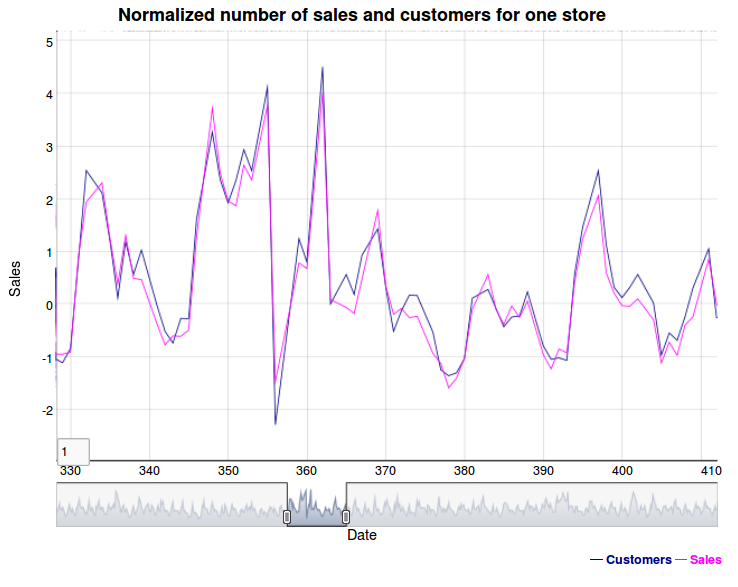
\includegraphics[width=\linewidth]{rossmann_visualization_sales-customers}
        \caption{Visualization of the Rossmann data for one store. Sales and number of customers are normalized.}
        \label{fig:sub1}
        \end{figure}

    \begin{figure}[H]
        \centering
        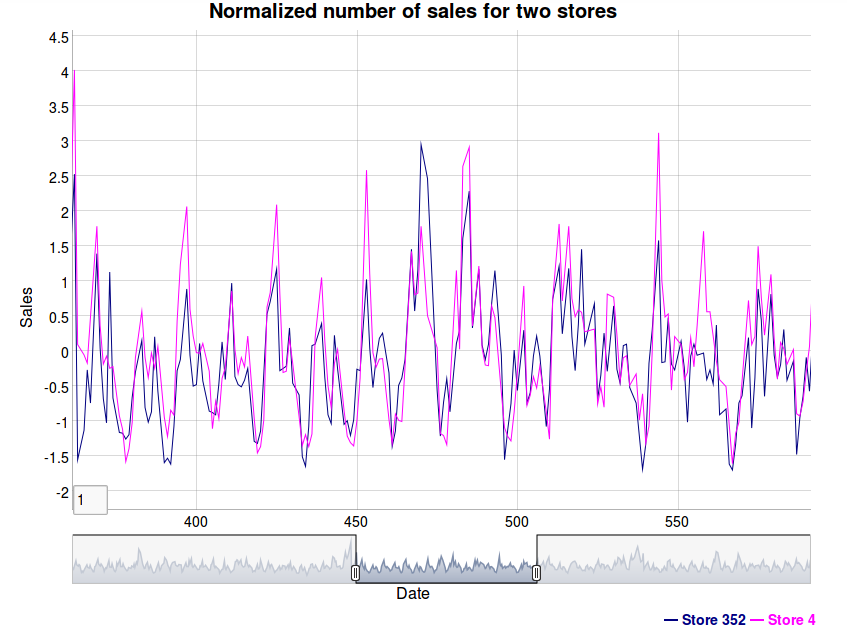
\includegraphics[width=\linewidth]{rossmann_visualization_two-stores}
        \caption{Visualization of the Rossmann data for two stores. Number of sales is normalized.}
        \label{fig:sub1}
    	\end{figure}

	\subsection{Time-independent features}
	Additional static information is provided for each store:

    \begin{figure}[H]
        \centering
	    \begin{tabular}{llp{2.7cm}}
	    \toprule
	    Feature & Type & Description\\
	    \toprule
	    StoreType		& categorical 	& four store models (a, b, c, d) \\
	    Assortment		& float 	 	& assortment level (a, b, c) \\
	    Comp. Distance
	     				& float 		& distance to nearest competing store in km \\
	    Comp. OpenSince
	     				& integer 		& month and year when nearest competitor opened \\
	    Promo2			& boolean		& whether the store is running a continuous promotion \\
	    Promo2Since 	& integer 		& week and year when the continuous promotion began \\
	    PromoInterval	& list of int & months when the promotion is started anew (unused) \\
	    \bottomrule
	    \end{tabular}
        \caption{Features from the store set}
	    \end{figure}

\section{Preprocessing}
\subsection{Missing values}
Only three stores are missing CompetitionDistance feature, but 354 stores does not have data for their nearest competitor's time of opening, and 544 stores does not have a starting date for Promo2 because they did not participate in the continuous promotion.

Due to time limitation, missing values for competitor's time of opening and time since Promo2 began are filled with zeros. \href{https://www.researchgate.net/post/Is_it_possible_to_train_a_neural_network_with_missing_data2}{Postings from ResearchGate} suggest using machine learning to guess the missing values, which is a possible next step for this project.

\subsection{Additional features}
Week and year when the store began the continuous promotion are combined into weeks since Promo2 began, as feature Promo2WeeksSinceJoined. Month and year when the nearest competing store was opened are combined into months since the competitor's opening, as feature CompetitionMonthsSinceOpen.

Feature WeekOfYear and Year were added to the train set in order to capture the seasonal sale pattern (i.e. the number of sales increases around Christmas), as suggested by Yang and Liu in their \href{http://cs229.stanford.edu/proj2015/215_report.pdf}{project report} on the dataset.

Store IDs are also used as a feature in order for the network to better recognize different stores while combining data from multiple stores for training.

\subsection{Normalization}
The Store IDs, Promo2WeeksSinceJoined, and CompetitionMonthsSinceOpen are all normalized to have mean zero and standard deviation of 1, whereas Sales and Customers features are normalized to be between 0 and 1 in order to use the sigmoid activation function, as suggested from \href{https://www.researchgate.net/post/Which_activation_function_should_be_used_in_a_prediction_model}{ResearchGate forum}. Initially the Sales and Customers values are normalized separately for each store. However, in order to use data from multiple stores on the same model, these features are normalized across the whole data set.

\section{The model}
\subsection{Recurrent Neural Networks}
Recurrent Neural Networks are a powerful dynamic modeling technique that have been applied to many time series problem such as music , text, motion capture or generating sequences. Time dependency is captured by sampling from the network's output distribution, then feeding the sample as input for the next time step, which also theoretically allows for prediction infinitely into the future \cite{DBLP:journals/corr/Graves13}.

In practice, however, RNN suffer from the vanishing gradients problem as the model back-propagates through time, making it unable from storing information for a long time.

\subsection{Long Short-Term Memory}
LSTM, first introduced by Hochreiter and Schmidhuber in 1997 \cite{Hochreiter:1997:LSM:1246443.1246450}, alleviates the vanishing gradients problem through using a memory cell for the hidden layer function, instead of the sigmoid function commonly used in other RNN architectures, with input, output and forget gates to essentially store memory better \cite{DBLP:journals/corr/Graves13}.

\section{Experiment}
The model is implemented using Keras on top of the Theano library in Python. A subset of 15 stores are selected randomly from the 1,115 stores for training and testing. Time-independent inputs are fed in to the network as constant values. There are in total 13 input features over 942 time steps for each store. The network's output are the number of sales and customers of the stores.

The model consists of one LSTM RNN layer provided by Keras with a fully connected layer for reducing the 13-dimension input to the 2-dimension output. After the LSTM layer, a 20\% dropout is implemented prevent over-fitting, as suggested by Srivastava et al. \cite{srivastava14-dropout}. For continuous value prediction, sigmoid activation was used with a meas squared error loss function. The network is optimized using the RMSPROP algorithm.
\begin{figure}[H]
    \centering
    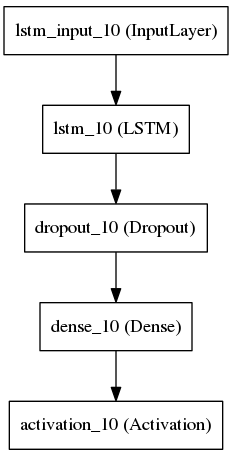
\includegraphics[width=0.7\linewidth]{model}
    \caption{Model of the LSTM RNNs}
    \label{fig_model}
	\end{figure}

The network is trained one store at a time, each for 5 epochs and 20\% of the data left out for validation, to find out if it can generalize to all stores using the static information from the store data set. However, it seems the validation accuracy does not strictly increase as the network is trained with more stores.

\begin{figure}[H]
    \centering
    \begin{tabular}{lc}
	    \toprule
	    Store 	& Validation accuracy (\%)\\
	    \toprule
	    854		& 88.36 	\\
	    1022	& 64.02 	\\
	    463		& 82.54		\\
	    905		& 93.65 	\\
	    494		& 99.47		\\
	    320 	& 86.24		\\
	    45		& 100.00	\\
	    \bottomrule
	    \end{tabular}
	\end{figure}

\begin{figure}[H]
    \centering
    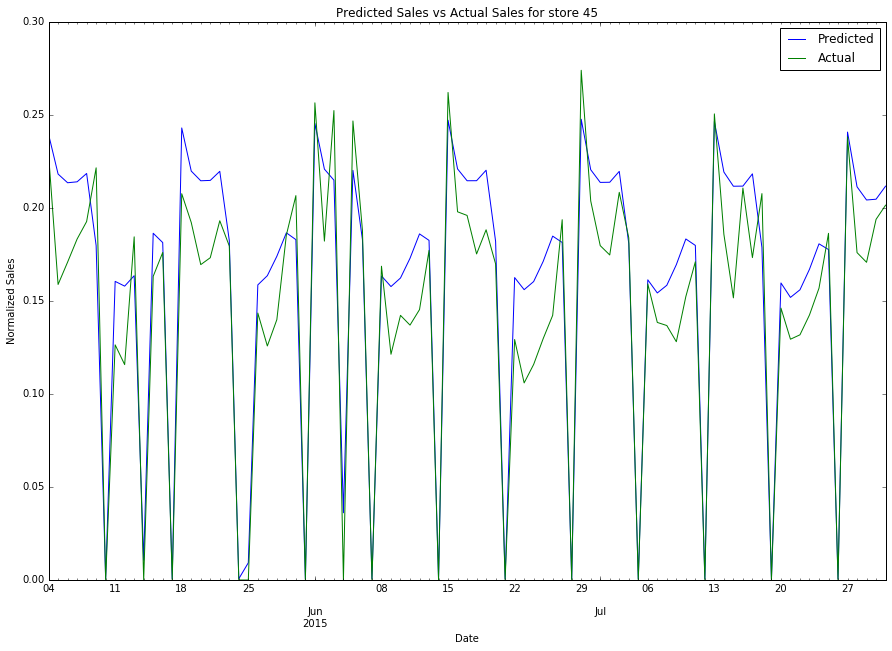
\includegraphics[width=0.9\linewidth]{rossmann_prediction_errors_store45}
    \caption{Prediction error of the normalized sales for store 45}
    \label{fig_pred_45}
	\end{figure}

\begin{figure}[H]
    \centering
    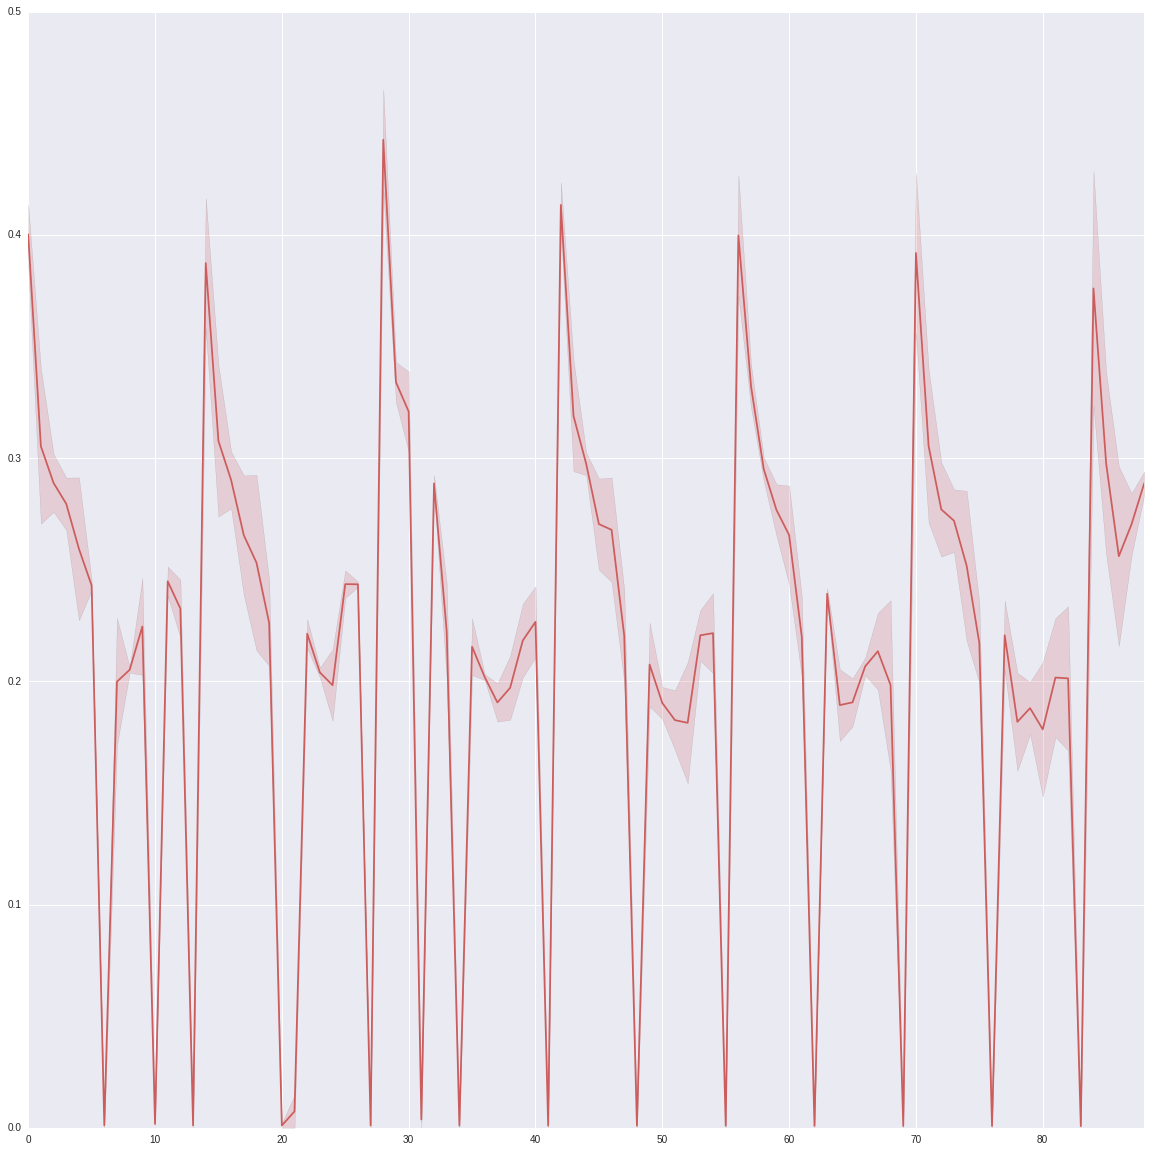
\includegraphics[width=0.9\linewidth]{rossmann_prediction_errors_store1022}
    \caption{Prediction error of the normalized sales for store 1022}
    \label{fig:sub2}
	\end{figure}

\section{Conclusion}
As the competition results are on the test data set and require submission to Kaggle, there's not a sound way to compare this model to State-of-the-art approaches. Additionally, given the time limitation, there remain many possible modifications to the LSTM model to be explored, which may further improve prediction performance. Firstly, a machine learning approach to filling missing values in the store data can be implemented. Secondly, experimentation with more hidden units, more layers or combination of layers may also allow the network to adapt to more stores. It would also be interesting to implement Gated Recurrent Unit (GRU), another popular variance of RNN, instead of LSTM. A more careful study into how Keras implement LSTM, loss function and activation function may also be required to fully understand whether the model is behaving as desired.

\bibliographystyle{plain}
\bibliography{../../RnD/RnD_sources.bib}

\end{document}
